%\begin{figure}[t]
%\centering
%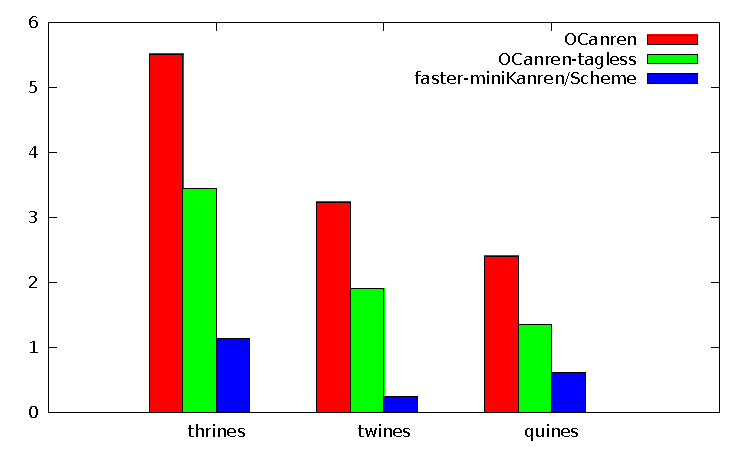
\includegraphics{graph2.pdf}
%\caption{The Second Set of Benchmarks}
%\label{eval:second}
%\end{figure}

\section{Performance Evaluation}
\label{sec:evaluation}

One of our initial goals was to evaluate, what performance impact would choosing OCaml as a host language make. In addition we spent some 
efforts in order to implement \miniKanren in an efficient, tagless manner, and, of course, the outcome of this decision also has to be 
measured. For comparison we took faster-miniKanren\footnote{\url{https://github.com/webyrd/faster-miniKanren}}~--- a full-fledged 
\miniKanren implementation for Scheme/Racket. It turned out that faster-miniKanren implements a number of optimizations~\cite{WillThesis, Optimizations} 
to speedup the search; moreover, the search order in our implementation initially was a little bit different. In order to make the comparison
fair, we additionally implemented all these optimizations and adjusted the search order to exactly coincide with 
what faster-miniKanren does.

\begin{figure}[t]
\centering
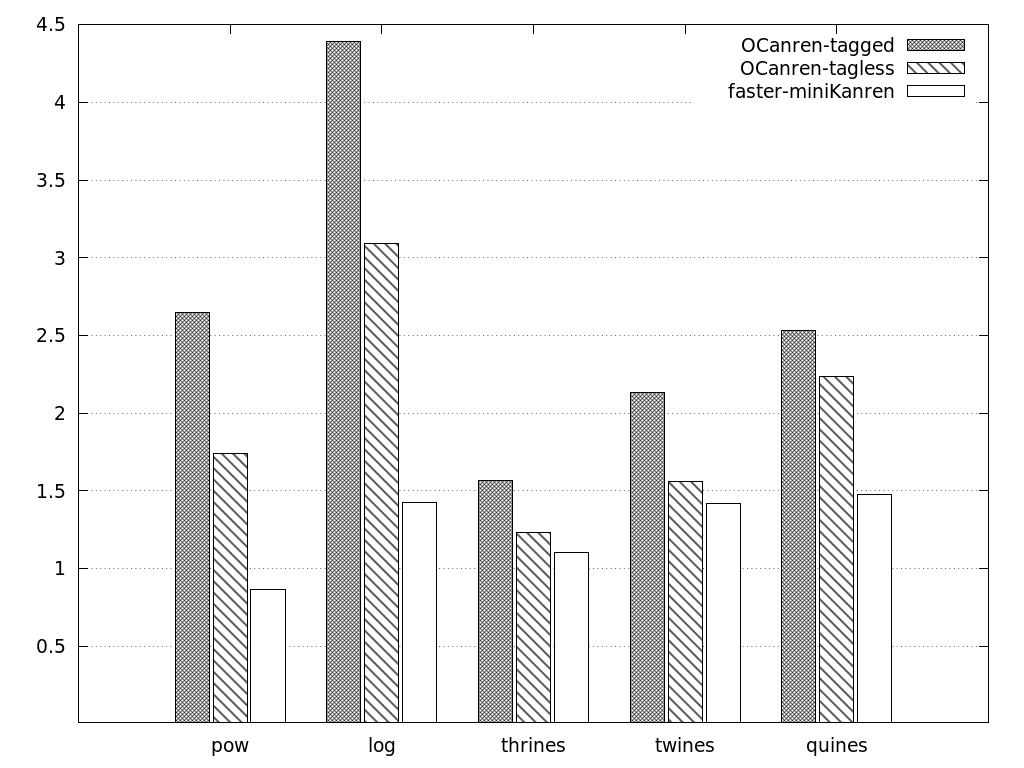
\includegraphics[scale=0.4]{graph.png}
\caption{The Results of the Performance Evaluation}
\label{eval}
\end{figure}

\FloatBarrier 

For the set of benchmarks we took the following problems:

\begin{itemize}
%\item \textbf{sorto, permo}~--- sorting and permutation for lists of Peano numbers (shown as example in Section~\ref{sec:examples}).
%The concrete tests are the sorting of the list \lstinline{[3; 2; 1; 0]} and taking all permutations of the list \lstinline{[0; 1; 2; 3; 4; 5; 6; 7]}.
\item \textbf{pow, logo}~--- exponentiation and logarithm for integers in binary form. The concrete tests relationally computed
$3^5$ (which is 243) and $log_3 243$ (which is, conversely, 5).
\item \textbf{quines, twines, trines}~--- self/co-evaluating program synthesis problems from~\cite{Untagged}. The
concrete tests took the first 100, 15 and 2 answers for these problems respectively.
\end{itemize}

%Since the last bundle of benchmarks uses disequality constraints (and, hence, $\mu$Kanren is ruled out) we
%split all benchmarks into two sets.

The evaluation was performed on a desktop computer with Intel Core i7-4790K CPU @ 4.00GHz processor and 16GB of memory.
For OCanren \mbox{ocaml-4.04.0+frame_pointer+flambda} was used, for faster-miniKanren~--- Chez~Scheme~9.4.1.
All benchmarks were ran in the natively compiled mode ten times, then average user time was taken. The results of the evaluation
are shown on Figure~\ref{eval}. The whole evaluation repository with all scripts and detailed description is accessible 
from \lstinline{GitHub}\footnote{\url{https://github.com/Kakadu/ocanren-perf}}.

The first conclusion, which is rather easy to derive from the results, is that the tagless approach indeed matters. Our initial
implementation did not show essential speedup in comparison even with $\mu$Kanren (and was even \emph{slower} on the logarithm
and permutations benchmarks). The situation was improved drastically, however, when we switched to the tagless version.

Yet, in comparison with faster-miniKanren our implementation is still lagging behind. We can conclude, that the optimizations, 
used in Scheme/Racket version, have a different impact in the OCaml case; we save this problem for future research.

